\documentclass[conference]{IEEEtran}

\usepackage[utf8]{inputenc}
\usepackage[T1]{fontenc}
\usepackage[spanish]{babel}
\usepackage{amsmath,amssymb}
\usepackage{graphicx}
\usepackage{booktabs}
\usepackage{cite}
\usepackage{url}

\begin{document}
	
	% Valores de pc y pm elegidos en el ajuste (los imprime la celda "GA = GAParams(...)" del cuaderno 03).
	\newcommand{\pcsel}{\textbf{[PC]}}
	\newcommand{\pmsel}{\textbf{[PM]}}
	
	\title{Comparación de Algoritmo gen\'etico frente a GRASP para extracci\'on de m\'etricas en fichas de modelos de Hugging Face}
	
	\author{\IEEEauthorblockN{Juan Felipe Gallo}
		\IEEEauthorblockA{Maestr\'ia en Ingenier\'ia, Universidad de Antioquia, Medell\'in, Colombia\\
			Metaheur\'istica 2026-01, Entrega 4}}
	
	\maketitle
	
	\begin{abstract}
		Se implementa un algoritmo gen\'etico (AG) para configurar la etapa de extracción de métricas de performance de modelos IA en un \emph{pipeline} ETL   para determinar cuáles son las reglas a activar, en qué orden y con qu\'e umbral, para maximizar el $F_1$ macro por tarea con a lo sumo $K$ reglas y precisi\'on m\'inima de 0,90. El AG se ajusta con una base de 18 configuraciones y 10 r\'eplicas, y se compara con el GRASP de la entrega anterior, un voraz constructivo y una b\'usqueda aleatoria, con 30 r\'eplicas y el mismo presupuesto, mediante pruebas no paramétricas como Kruskal--Wallis, Mann--Whitney con correcci\'on de Holm, Friedman y Wilcoxon pareado. Con $K=5$ y $K=6$ el voraz, GRASP y el AG alcanzan el mismo valor (0,3401 y 0,3572); GRASP lo reproduce en las 60 r\'eplicas, el AG en 51 de 60 y la b\'usqueda aleatoria en ninguna. La diferencia entre el AG y GRASP es estad\'isticamente detectable pero pequeña, como m\'aximo de 0,009. El voraz llega al mismo valor con 367 evaluaciones frente a unas 3.100 de GRASP. En validaci\'on cruzada por organizaci\'on los tres m\'etodos coinciden en los cinco pliegues. Solo el tamaño de población influye en el AG: óptimo en el 88 \% de las corridas con N=100 y en el 48 \% con N=30, a cambio de más evaluaciones. Como el voraz ya obtiene el óptimo, en esta instancia las metaheurísticas solo pueden igualarlo.
	\end{abstract}
	
	\begin{IEEEkeywords}
		algoritmo gen\'etico, GRASP, pruebas no param\'etricas, extracci\'on de informaci\'on, optimizaci\'on combinatoria.
	\end{IEEEkeywords}
	
	\section{Implementaci\'on}
	
	\subsection{Problema y base de la Entrega 3}
	Durante la estapa de extracción del ETL\cite{repo}, sólo se leen los metadatos estandarizados que provienen de la documentación de Hugging Face. Cada ficha de modelo (\emph{model card}) \cite{mitchell} puede traer m\'etricas en el bloque \texttt{model-index} y en tablas y l\'ineas del cuerpo. Se configura una etapa de recuperaci\'on sobre el cuerpo: una soluci\'on es $x=(\pi,\theta)$, con $\pi$ una tupla ordenada de a lo sumo $K$ reglas distintas de un cat\'alogo de $m=27$, es decir, 3 analizadores $\times$ 9 familias de m\'etricas y un $\theta\in\{1,100,1000\}$ una cota de plausibilidad. Para cada ficha y m\'etrica, la primera regla de $\pi$ que la produce gana. La aptitud es el $F_1$ macro por \texttt{pipeline\_tag} sobre 390 fichas con referencia que se encuentra oculto en el \texttt{model-index}, con restricciones duras de precisi\'on $P\ge0{,}90$ y, opcionalmente, de tiempo por ficha: $f(x)=\bar F_1(x)$ si es factible y $-1-v(x)$ si no. Las salidas de las reglas se precalculan, de modo que evaluar una configuraci\'on cuesta 3,3\,ms, y una cach\'e guarda cada configuraci\'on evaluada: el presupuesto cuenta solo evaluaciones reales. Esta Entrega reutiliza esa infraestructura, el vecindario de cinco movimientos (insertar, eliminar, reemplazar, intercambiar, cambiar $\theta$) y la construcci\'on aleatorizada de GRASP \cite{feo}.
	
	\subsection{Algoritmo gen\'etico}
	La implementaci\'on sigue el dise\~no de la Entrega 2 \cite{gendreau,goldberg} y est\'a en el m\'odulo \texttt{genetic}; \texttt{stats} contiene las pruebas estad\'isticas y \texttt{experiments} los protocolos de comparaci\'on, ajuste y validaci\'on cruzada. Los componentes son:
	
	\textbf{Poblaci\'on inicial.} Una fracci\'on $\rho$ de los $N$ individuos se construye con la construcci\'on aleatorizada de GRASP ($\alpha=0{,}3$); el resto son aleatorios, con tama\~no uniforme en $\{1,\dots,K\}$, reglas distintas y $\theta$ al azar. Los duplicados se descartan.
	
	\textbf{Selecci\'on.} Torneo de tama\~no $k_t=3$ sobre la aptitud $f$; las soluciones infactibles quedan por debajo de las factibles.
	
	\textbf{Cruce.} Cruce por orden \cite{davis}: el hijo conserva un prefijo del padre $a$ (corte aleatorio) y se completa con las reglas del padre $b$ que faltan, en el orden de $b$, hasta $K$; $\theta$ se hereda de uno de los dos padres. Se aplica con probabilidad $p_c$.
	
	\textbf{Mutaci\'on.} Con probabilidad $p_m$ se aplica un movimiento aleatorio del vecindario, el mismo de GRASP. Si el hijo ya est\'a en la poblaci\'on nueva, se muta de nuevo hasta 5 veces.
	
	\textbf{Reemplazo y memoria.} Generacional con elitismo ($e=2$). La cach\'e es la de GRASP, y el presupuesto cuenta evaluaciones reales.
	
	\textbf{Parada.} Se agota el presupuesto $B$ o la mejor aptitud no mejora en $G$ generaciones consecutivas.
	
	\begin{table}[t]
		\centering
		\caption{Par\'ametros del AG: diseño y valor usado}
		\label{tab:params}
		\footnotesize
		\begin{tabular}{lcc}
			\toprule
			Par\'ametro & Rango / dise\~no & Usado \\
			\midrule
			$N$ (poblaci\'on) & $\{30,50,100\}$ & 100 \\
			$p_c$ & $\{0{,}7;0{,}9\}$ & \pcsel \\
			$p_m$ & $\{0{,}1;0{,}2;0{,}4\}$ & \pmsel \\
			$k_t$, $e$, $\rho$, $G$ & 3, 2, 0,2, 15 & sin cambios \\
			$B$ (evaluaciones) & 3.000 & 3.000 \\
			\bottomrule
		\end{tabular}
	\end{table}
	
	\subsection{Desviaciones respecto al diseñoo}
	La siembra con GRASP no puede gastar m\'as del 25\,\% del presupuesto: una construcci\'on cuesta unas 365 evaluaciones con $K=5$ y $\rho N=20$ construcciones agotar\'ian el presupuesto antes de la primera generaci\'on. En la pr\'actica solo se siembran los que caben en ese tope. La parada por estancamiento ($G=15$) puede detener al AG antes de agotar el presupuesto.$k_t$, $e$, $\rho$ y $G$ se fijaron en los valores iniciales sin ajustarlos.
	
	\section{Experimentos}
	
	\subsection{Instancia y m\'etodos}
	Se usa la instancia del cat\'alogo completo de la Entrega 3: 27 reglas, 390 fichas de referencia, $K\in\{5,6\}$ y sin l\'imite de tiempo. Se comparan cuatro m\'etodos: voraz constructivo, b\'usqueda aleatoria, GRASP ($\alpha=0{,}3$) y AG, los tres \'ultimos con presupuesto de 3.000 evaluaciones. En el caso de GRASP, no se interrumpe una construcción ni un barrido del vecindario al llegar al presupuesto, y por eso lo excede con una media de 3.089 y 3.146 evaluaciones; m\'aximo 3.434, y la b\'usqueda aleatoria toma 3.000 muestras, de las cuales solo unas 2.400 son configuraciones distintas.
	
	\subsection{Ajuste del AG}
	Base completa $N\times p_c\times p_m$ de 18 configuraciones, 10 r\'eplicas por configuraci\'on con semillas 1000--1009, $K=5$. El ajuste usa la misma instancia que la comparaci\'on final, con semillas distintas.
	
	\subsection{Comparaci\'on y validaci\'on cruzada}
	Comparaci\'on con 30 r\'eplicas con semillas 0--29 para $K=5$ y $K=6$. Validaci\'on cruzada con 5 pliegues por organizaci\'on, equilibrados por fichas (236, 39, 39, 38 y 38): en cada pliegue se optimiza con los otros cuatro y se mide en el reservado ($K=5$), sin l\'imite de tiempo, 10 r\'eplicas por m\'etodo.
	
	\section{An\'alisis de desempe\~no y ajuste de par\'ametros}
	
	\subsection{Prop\'osito y elecci\'on de las pruebas}
	A partir de las pruebas, se decide si los par\'ametros del AG afectan su desempeño, y se comparan los algoritmos de las Entregas 3 y 4. Se usan pruebas no param\'etricas porque muchas r\'eplicas devuelven exactamente el mismo valor, con varianza nula en GRASP, 10 a 30 observaciones por grupo, lo que no permite suponer normalidad ni homogeneidad de varianzas, como exigir\'ia un ANOVA.
	\begin{itemize}
		\item \textbf{Kruskal--Wallis} \cite{kruskal}: compara $k$ grupos independientes. Se usa para el ajuste 18 configuraciones, cada par\'ametro por separado y para los tres m\'etodos estoc\'asticos.
		\item \textbf{Mann--Whitney} \cite{mann} con correcci\'on de Holm \cite{holm}: comparaciones por pares entre m\'etodos. Las semillas de un m\'etodo no est\'an emparejadas con las de otro, de modo que las r\'eplicas son independientes. El tama\~no de efecto es $\delta$ de Cliff \cite{cliff}, $P(A>B)-P(A<B)$.
		\item \textbf{Wilcoxon de una muestra} contra el valor fijo del voraz determinista, con Holm.
		\item \textbf{Friedman} \cite{friedman,demsar} y \textbf{Wilcoxon pareado} con Holm en la validaci\'on cruzada, donde los pliegues s\'i son bloques reales; se agrega cada pliegue con la mediana de sus r\'eplicas.
	\end{itemize}
	La implementación se realizó en la librera SciPy \cite{scipy} de Python; la correcci\'on de Holm, el $\delta$ de Cliff y los intervalos \emph{bootstrap} con 10.000 remuestreos est\'an en el m\'odulo \texttt{stats}. Se usa $\alpha=0{,}05$ y los valores $p$ son bilaterales.
	
	\subsection{Ajuste de par\'ametros}
	La Tabla~\ref{tab:ajuste} resume el ajuste por tama\~no de poblaci\'on. El \'optimo de la instancia ($K=5$) es 0,3401. Kruskal--Wallis entre las 18 configuraciones da $H=37{,}4$ ($p=0{,}003$). Por par\'ametro, el tama\~no de poblaci\'on es el \'unico con efecto ($H=26{,}1$, $p<0{,}001$), mientras que $p_c$ ($H=0{,}06$; $p=0{,}81$) y $p_m$ ($H=0{,}05$; $p=0{,}97$) no tienen efecto detectable. Las cuatro configuraciones con $N=100$ y $p_m\ge0{,}2$ alcanzan 0,3401 en las 10 r\'eplicas. Se fij\'o $N=100$ y, entre esas cuatro, $p_c=\pcsel$ y $p_m=\pmsel$, que son estad\'isticamente equivalentes.
	
	El costo de la mejora con $N$ es de 1.469 a 2.430 evaluaciones y de 2,9 a 5,3\,s por corrida. Adem\'as, el efecto est\'a confundido con el criterio de parada: $G$ se mide en generaciones, y una poblaci\'on mayor eval\'ua m\'as configuraciones antes de declarar estancamiento. Con el dise\~no actual no es posible separar ambos efectos.
	
	\begin{table}[t]
		\centering
		\caption{Ajuste del AG por tama\~no de poblaci\'on ($K=5$; 6 configuraciones $\times$ 10 semillas = 60 corridas por fila)}
		\label{tab:ajuste}
		\footnotesize
		\begin{tabular}{lcccc}
			\toprule
			$N$ & Media $\bar F_1$ & En el \'optimo & Evaluaciones & Segundos \\
			\midrule
			30 & 0,3346 & 48\,\% & 1.469 & 2,9 \\
			50 & 0,3379 & 55\,\% & 1.789 & 3,7 \\
			100 & 0,3398 & 88\,\% & 2.430 & 5,3 \\
			\bottomrule
		\end{tabular}
	\end{table}
	
	\subsection{Comparaci\'on de los algoritmos}
	La Tabla~\ref{tab:comp} muestra los resultados con 30 r\'eplicas. Kruskal--Wallis entre los tres m\'etodos estoc\'asticos rechaza la igualdad ($K=5$: $H=77{,}6$; $K=6$: $H=78{,}6$; ambos $p<10^{-16}$), y el origen es la b\'usqueda aleatoria. La Tabla~\ref{tab:pares} detalla los pares.
	
	\begin{table}[t]
		\centering
		\caption{Comparaci\'on con 30 r\'eplicas, cat\'alogo completo y  sin límite de tiempo.}
		\label{tab:comp}
		\footnotesize
		\setlength{\tabcolsep}{3.5pt}
		\begin{tabular}{llcccccc}
			\toprule
			$K$ & M\'etodo & Mediana & Media$\pm$DE & M\'in. & Mejor & Eval. & s \\
			\midrule
			5 & Voraz & 0,3401 & 0,3401 & 0,3401 & -- & 367 & 1,1 \\
			& Aleatoria & 0,2918 & 0,2935$\pm$0,0165 & 0,2642 & 0/30 & 2.394 & 2,3 \\
			& GRASP & 0,3401 & 0,3401$\pm$0,0000 & 0,3401 & 30/30 & 3.089 & 6,5 \\
			& AG & 0,3401 & 0,3395$\pm$0,0023 & 0,3309 & 25/30 & 2.393 & 5,5 \\
			\midrule
			6 & Voraz & 0,3572 & 0,3572 & 0,3572 & -- & 499 & 1,4 \\
			& Aleatoria & 0,3149 & 0,3125$\pm$0,0147 & 0,2846 & 0/30 & 2.517 & 2,4 \\
			& GRASP & 0,3572 & 0,3572$\pm$0,0000 & 0,3572 & 30/30 & 3.146 & 7,4 \\
			& AG & 0,3572 & 0,3568$\pm$0,0017 & 0,3485 & 26/30 & 2.512 & 6,6 \\
			\bottomrule
		\end{tabular}
	\end{table}
	
	\begin{table}[t]
		\centering
		\caption{Pruebas por pares: $p$ ajustado por Holm y $\delta$ de Cliff}
		\label{tab:pares}
		\footnotesize
		\begin{tabular}{lcccc}
			\toprule
			& \multicolumn{2}{c}{$K=5$} & \multicolumn{2}{c}{$K=6$} \\
			Comparaci\'on & $p_{\text{Holm}}$ & $\delta$ & $p_{\text{Holm}}$ & $\delta$ \\
			\midrule
			AG vs GRASP & 0,022 & $-0{,}17$ & 0,042 & $-0{,}13$ \\
			AG vs Aleatoria & $<10^{-10}$ & $+1{,}00$ & $<10^{-10}$ & $+1{,}00$ \\
			GRASP vs Aleatoria & $<10^{-11}$ & $+1{,}00$ & $<10^{-11}$ & $+1{,}00$ \\
			AG vs Voraz & 0,077 & $-0{,}17$ & 0,131 & $-0{,}13$ \\
			GRASP vs Voraz & 1,000 & 0,00 & 1,000 & 0,00 \\
			Aleatoria vs Voraz & $<10^{-5}$ & $-1{,}00$ & $<10^{-5}$ & $-1{,}00$ \\
			\bottomrule
		\end{tabular}
	\end{table}
	
	\emph{GRASP y el AG superan a la b\'usqueda aleatoria} en todas las r\'eplicas ($\delta=+1$), con el mismo presupuesto. \emph{GRASP no se distingue del voraz}: reproduce su valor en las 60 r\'eplicas. \emph{El AG es peor que GRASP} ($p=0{,}022$ y $0{,}042$), pero la diferencia es de efecto peque\~no ($|\delta|\le0{,}17$, mediana de diferencia nula) y de magnitud m\'axima 0,009. La proporci\'on de r\'eplicas que alcanzan el mejor valor (AG 51/60, GRASP 60/60) tambi\'en difiere (Fisher exacta, $p=0{,}003$, agrupando $K=5$ y $K=6$). Frente al voraz, la diferencia del AG deja de ser significativa tras corregir por comparaciones múltiples (p de Holm = 0,077 y 0,131).
	
	\subsection{Validaci\'on cruzada}
	La Tabla~\ref{tab:cv} muestra la mediana por pliegue de las 10 r\'eplicas. El voraz, GRASP y el AG dan el mismo valor en los cinco pliegues; la b\'usqueda aleatoria es peor en tres y coincide en dos. Friedman rechaza la igualdad ($\chi^2=9{,}0$, 3 gl, $p=0{,}029$), pero solo por la aleatoria (rangos medios 3,4 frente a 2,2 de los otros tres). En las comparaciones pareadas ning\'un par es significativo: con solo tres pliegues con diferencia, el menor $p$ posible de Wilcoxon es 0,25 y con Holm todos valen 1; la mediana de la diferencia voraz--aleatoria es 0,046 (IC bootstrap 95\,\%: 0,000--0,085). El desempe\~no fuera de muestra var\'ia de 0,21 a 0,54 seg\'un el pliegue, mucho m\'as que cualquier diferencia entre m\'etodos.
	
	\begin{table}[t]
		\centering
		\caption{Validaci\'on cruzada por organizaci\'on, $K=5$, mediana de 10 r\'eplicas del $\bar F_1$ en el pliegue reservado}
		\label{tab:cv}
		\footnotesize
		\begin{tabular}{lccccc}
			\toprule
			Pliegue & Fichas & Voraz & Aleatoria & GRASP & AG \\
			\midrule
			0 & 236 & 0,538 & 0,538 & 0,538 & 0,538 \\
			1 & 39 & 0,243 & 0,243 & 0,243 & 0,243 \\
			2 & 39 & 0,206 & 0,157 & 0,206 & 0,206 \\
			3 & 38 & 0,368 & 0,322 & 0,368 & 0,368 \\
			4 & 38 & 0,402 & 0,317 & 0,402 & 0,402 \\
			\midrule
			Media & & 0,351 & 0,315 & 0,351 & 0,351 \\
			\bottomrule
		\end{tabular}
	\end{table}
	
	\section{Resultados adicionales}
	
	\subsection{Convergencia}
	La Fig.~\ref{fig:conv} muestra la mejor aptitud acumulada promedio. La curva del AG empieza cerca de las 1.000 evaluaciones, porque, seg\'un la figura, la poblaci\'on inicial con la siembra de GRASP consume cerca de un tercio del presupuesto antes de la primera generaci\'on; sube hasta una meseta cercana a 0,3395, $K=5$, hacia las 2.150 evaluaciones y 0,3568, $K=6$, hacia las 2.300, siempre por debajo del valor del voraz. La curva de GRASP queda oculta bajo la l\'inea punteada del voraz: coincide con ella en todo el rango mostrado.
	
	\begin{figure}[t]
		\centering
		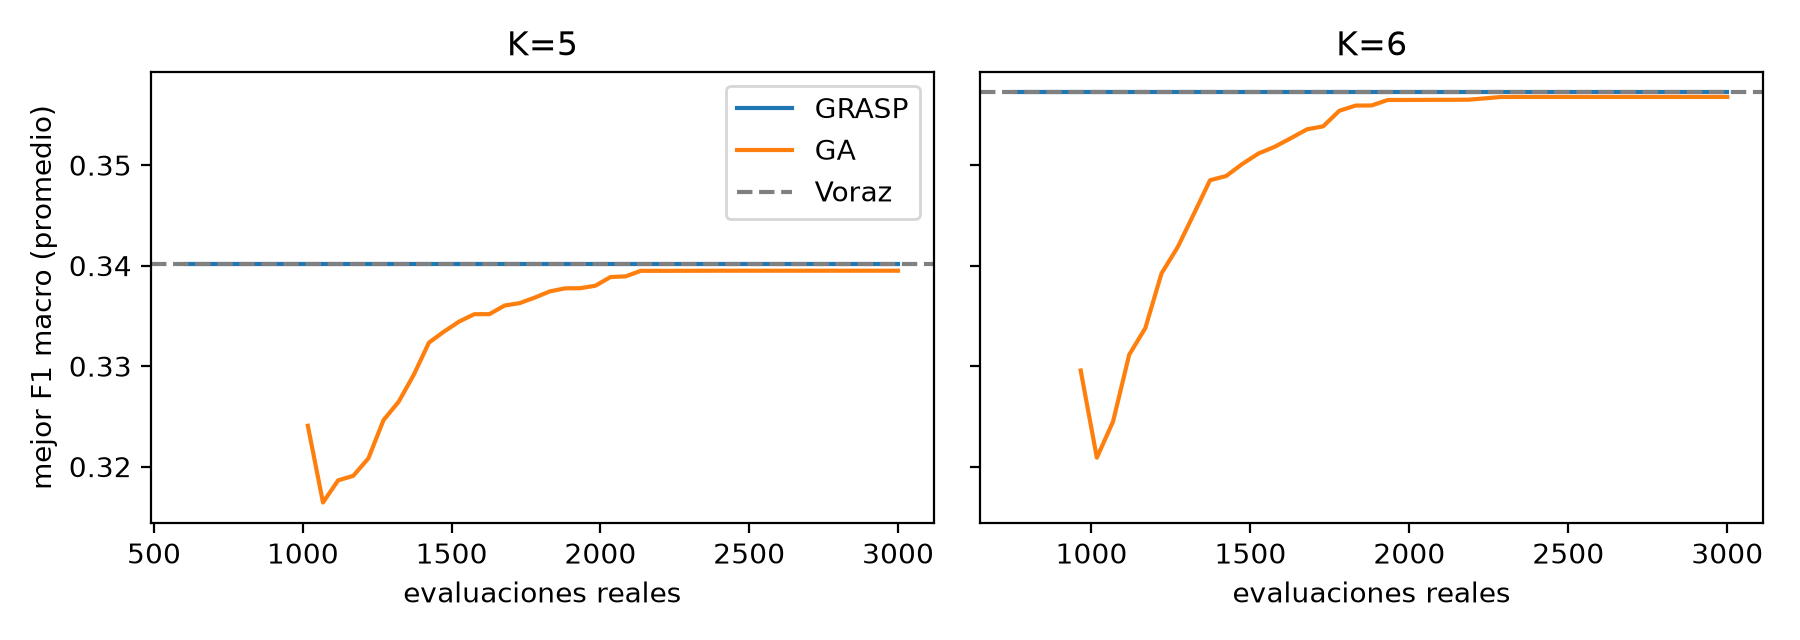
\includegraphics[width=\columnwidth]{convergencia_ga_grasp.png}
		\caption{Mejor $\bar F_1$ acumulado frente a evaluaciones reales. La curva de GRASP coincide con la l\'inea del voraz.}
		\label{fig:conv}
	\end{figure}
	
	\subsection{Estructura de las soluciones}
	Las 30 soluciones de GRASP con $K=5$ son el mismo conjunto de cinco reglas \texttt{clf\_basic} en l\'inea y en columna, \texttt{at\_k} en fila, \texttt{rouge} y \texttt{rank} en l\'inea, con 28 \'ordenes distintos y $\theta\in\{100,1000\}$. Con $K=6$ se a\~nade \texttt{clf\_avg} en l\'inea con un conjunto de 30 \'ordenes. El AG produce 3 y 4 conjuntos distintos, y todas sus corridas por debajo del \'optimo terminaron antes de agotar el presupuesto entre 1.909 y 2.658 evaluaciones: lo detuvo el criterio de estancamiento. Las tres corridas que agotaron las 3.000 evaluaciones alcanzaron el \'optimo.
	
	\subsection{Pliegue grande}
	En el pliegue 0 el cuál pertenece a la organizaci\'on dominante, 236 fichas, la soluci\'on \'optima en entrenamiento da 0,538 en prueba, y dos de las diez r\'eplicas del AG, con aptitud de entrenamiento algo menor (0,292 frente a 0,295), llegan a 0,683, y tres de las diez de la aleatoria superan 0,55. Son pocas r\'eplicas, pero indican que el \'optimo de entrenamiento no es el mejor fuera de muestra.
	

	\section{An\'alisis y conclusiones}
	
	En esta instancia las metaheur\'isticas no tienen c\'omo superar al voraz. El voraz constructivo alcanza con unos cientos de evaluaciones el mismo valor que GRASP y el AG obtienen con varios miles, y las soluciones de GRASP son siempre el mismo conjunto de reglas con \'ordenes y umbrales intercambiables. Con este cat\'alogo y estos valores de $K$, el problema se reduce a elegir un subconjunto de reglas, hay una meseta de \'optimos equivalentes en orden y umbral, y una b\'usqueda voraz ya la encuentra. Por eso la comparaci\'on entre los m\'etodos deja de ser una cuesti\'on de calidad y pasa a ser de fiabilidad y de costo.
	
	En términos de fiabilidad, GRASP supera el AG, ya que reproduce el mejor valor en todas las r\'eplicas, mientras que el AG se queda por debajo en algunas, con una diferencia estad\'isticamente detectable pero de magnitud m\'inima. El AG hace menos evaluaciones y gasta menos tiempo,por su criterio de parada que lo detiene por estancamiento antes de llegar al \'optimo, pues todas las corridas que agotaron el presupuesto lo alcanzaron.  El tamaño de población influye, pero una poblaci\'on mayor tambi\'en eval\'ua m\'as configuraciones antes de declarar estancamiento, de modo que con este dise\~no no puede separarse si ayuda por su diversidad o por su mayor esfuerzo de b\'usqueda y las probabilidades de cruce y de mutaci\'on no mostraron efecto alguno.
	
	Fuera de muestra, el voraz, GRASP y el AG dan el mismo resultado en todos los pliegues y solo la b\'usqueda aleatoria es peor en algunos. Con cinco pliegues, y solo tres con alguna diferencia, las pruebas pareadas carecen de potencia, as\'i que el resultado debe leerse como falta de evidencia y no como ausencia de diferencias.En dos de los cinco pliegues todos los m\'etodos dan el mismo resultado, de modo que solo tres sirven para compararlos, y en esos tres \'unicamente la b\'usqueda aleatoria sale peor. Con tres pliegues, la prueba de Wilcoxon no puede dar un resultado significativo aunque un m\'etodo gane en todos: su menor valor $p$ posible es 0,25. Por eso, que la prueba no encuentre diferencias no indica que los m\'etodos rindan igual, sino que hay muy pocos datos para saberlo.
	
	\begin{thebibliography}{99}
		\bibitem{mitchell} M. Mitchell \emph{et al.}, ``Model cards for model reporting,'' in \emph{Proc. Conf. Fairness, Accountability, and Transparency (FAT*)}, Atlanta, GA, USA, 2019, pp. 220--229.
		\bibitem{feo} T. A. Feo and M. G. C. Resende, ``Greedy randomized adaptive search procedures,'' \emph{J. Global Optim.}, vol. 6, no. 2, pp. 109--133, 1995.
		\bibitem{gendreau} M. Gendreau and J.-Y. Potvin, Eds., \emph{Handbook of Metaheuristics}, 3rd ed. Cham, Switzerland: Springer, 2019.
		\bibitem{goldberg} D. E. Goldberg, \emph{Genetic Algorithms in Search, Optimization, and Machine Learning}. Reading, MA, USA: Addison-Wesley, 1989.
		\bibitem{davis} L. Davis, ``Applying adaptive algorithms to epistatic domains,'' in \emph{Proc. 9th Int. Joint Conf. Artificial Intelligence (IJCAI)}, vol. 1, Los Angeles, CA, USA, 1985, pp. 162--164.
		\bibitem{kruskal} W. H. Kruskal and W. A. Wallis, ``Use of ranks in one-criterion variance analysis,'' \emph{J. Amer. Statist. Assoc.}, vol. 47, no. 260, pp. 583--621, 1952.
		\bibitem{mann} H. B. Mann and D. R. Whitney, ``On a test of whether one of two random variables is stochastically larger than the other,'' \emph{Ann. Math. Statist.}, vol. 18, no. 1, pp. 50--60, 1947.
		\bibitem{holm} S. Holm, ``A simple sequentially rejective multiple test procedure,'' \emph{Scand. J. Statist.}, vol. 6, no. 2, pp. 65--70, 1979.
		\bibitem{friedman} M. Friedman, ``The use of ranks to avoid the assumption of normality implicit in the analysis of variance,'' \emph{J. Amer. Statist. Assoc.}, vol. 32, no. 200, pp. 675--701, 1937.
		\bibitem{demsar} J. Dem\v{s}ar, ``Statistical comparisons of classifiers over multiple data sets,'' \emph{J. Mach. Learn. Res.}, vol. 7, pp. 1--30, 2006.
		\bibitem{cliff} N. Cliff, ``Dominance statistics: Ordinal analyses to answer ordinal questions,'' \emph{Psychol. Bull.}, vol. 114, no. 3, pp. 494--509, 1993.
		\bibitem{scipy} SciPy Community, ``scipy.stats.kruskal,'' \emph{SciPy Reference Guide}. [Online]. Available: \url{https://docs.scipy.org/doc/scipy/reference/generated/scipy.stats.kruskal.html}
		\bibitem{repo} J. F. Gallo, ``huggingface-etl-co2emissions,'' GitHub repository. [Online]. Available: \url{https://github.com/jufegare000/huggingface-etl-co2emissions}
	\end{thebibliography}
	
\end{document}